\chapter{जीनोमिकी और अनुक्रमण}\label{ch:b3:genomics}

किसी स्वतंत्रजीवी जीव का पहला पूर्ण जीनोम, किसी जीवाणु के \qty{1.8}{Mb},
चालीस लोगों की टोली के एक वर्ष के काम के बाद 1995 में प्रकाशित हुआ।
मानव जीनोम, \num{3.2} अरब क्षार युग्म, किसी अंतरराष्ट्रीय संघ को तेरह
वर्ष और लगभग तीन अरब डॉलर ले गया और 2003 में पूरा घोषित हुआ। आज कोई
मेज़ पर रखी मशीन कुछ सौ डॉलर में रात भर में मानव जीनोम पढ़ लेती है, कोई
अस्पताल औषध चुनने के लिए रोगी के अर्बुद का अनुक्रमण करता है, और कोई
संग्रहालय चालीस हज़ार वर्ष पुरानी किसी हड्डी का जीनोम निकालकर पढ़ लेता
है। जिस तकनीक ने यह संभव किया, जो गणित लाखों छोटे \omterm{def:b3:genomics:ngs}{वाचनों} को जीनोम में
बदलता है, और पूर्ण जीनोमों ने हमारे DNA के आकार, अंतर्वस्तु तथा इतिहास
के बारे में जो सिखाया है --- यही इस अध्याय का विषय है। उसके बाद का
अध्याय उन अल्गोरिद्मों को उठाता है जो हाथ में आ चुके अनुक्रमों की तुलना
करते हैं।

\section{DNA पढ़ना}

\begin{definition}[शृंखला-समापन से अनुक्रमण]\label{def:b3:genomics:sanger}
\index{सैंगर अनुक्रमण}\index{डाइडिऑक्सीन्यूक्लियोटाइड}\index{शृंखला-समापन}
\emph{सैंगर अनुक्रमण} किसी एकलड़ी साँचे की नकल किसी प्रारंभक से DNA
पॉलीमरेज़ द्वारा चारों सामान्य न्यूक्लियोटाइडों और
\emph{डाइडिऑक्सीन्यूक्लियोटाइडों} के एक छोटे अनुपात की उपस्थिति में
करता है, और इन डाइडिऑक्सी रूपों में 3$'$ हाइड्रॉक्सिल नहीं होता,
इसलिए वे जहाँ भी बैठते हैं शृंखला समाप्त कर देते हैं। हर
डाइडिऑक्सीन्यूक्लियोटाइड एक भिन्न प्रतिदीप्त रंजक ढोता है। उत्पाद
खंडों का ऐसा मिश्रण है जिसमें साँचे की हर स्थिति के लिए एक खंड है और
हर एक का अंत ज्ञात पहचान वाले क्षार पर होता है; जेल की किसी केशिका में
आकार से पृथक होकर वे लंबाई के क्रम में किसी संसूचक के आगे से गुज़रते
हैं, और रंगों का क्रम ही साँचे का अनुक्रम है। एक बारी में
\qtyrange{700}{900}{bp} $10^{-3}$ से कम त्रुटि-दर पर पढ़े जाते हैं; किसी
संरचना या किसी एक जीन की पुष्टि के लिए यही विधि बनी हुई है।
\end{definition}

\begin{proof}[प्रमाण-सामग्री]
सैंगर, निकलेन और कुल्सन ने यह विधि 1977 में प्रकाशित की और उसी वर्ष
उससे फ़ेज $\phi$X174 के \qty{5386}{bp} पढ़े --- पहला पूर्ण DNA जीनोम ---
और 1981 में मानव सूत्रकणिका के \qty{16569}{bp}। फ़्लाइशमैन और सहयोगियों
(1995) ने \emph{Haemophilus influenzae} के \qty{1.83}{Mb} पूरे जीनोम को
यादृच्छिक खंडों में तोड़कर, उनमें से \num{24000} का अनुक्रमण करके और
\omterm{def:b3:genomics:ngs}{वाचनों} को कंप्यूटर से जोड़कर पढ़े --- यही वह \emph{पूर्ण-जीनोम शॉटगन}
रणनीति है जिसे हर बाद की परियोजना ने और बड़ा किया।
\end{proof}

\begin{omfigure}
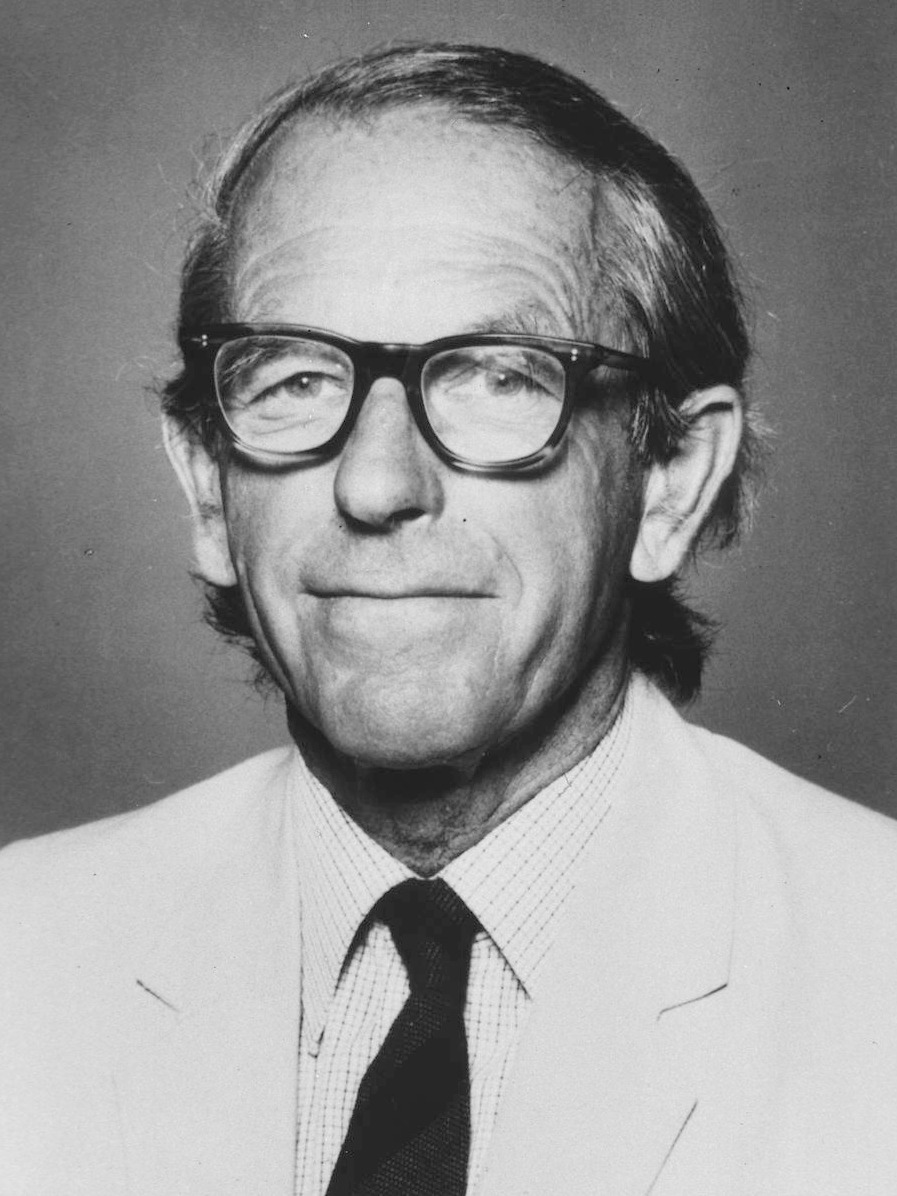
\includegraphics[width=0.30\linewidth]{images/book5/sanger.jpg}\hspace{0.04\linewidth}
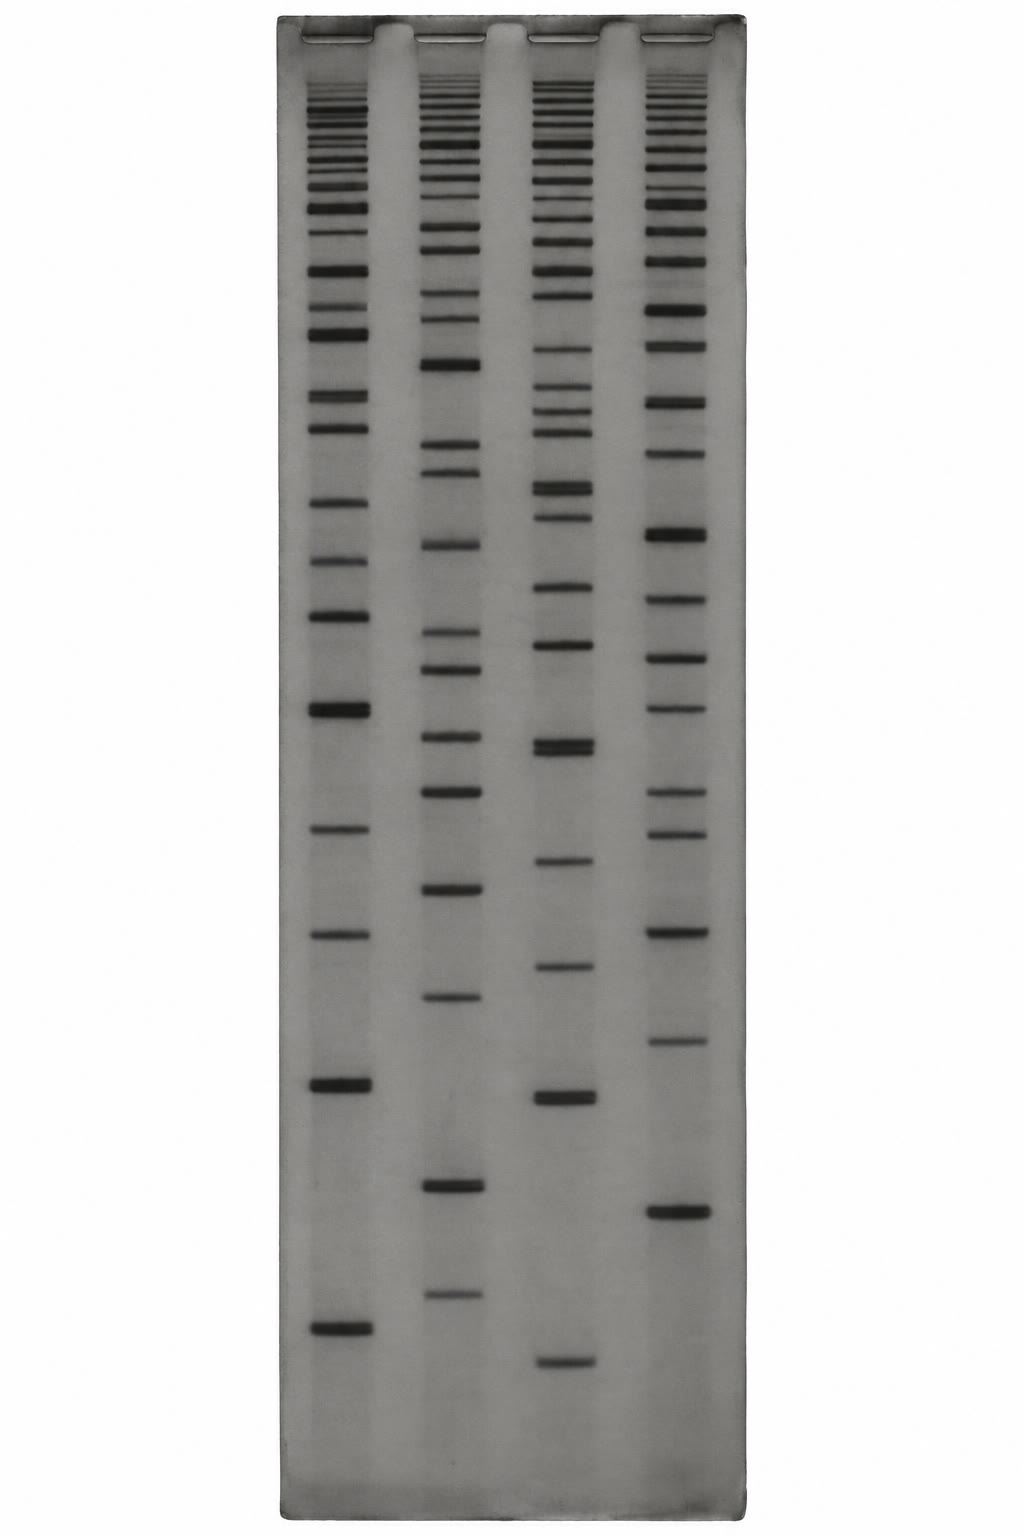
\includegraphics[width=0.30\linewidth]{images/book5/ai/b5-04-sanger-gel.jpg}

{\small बाएँ: फ़्रेडरिक सैंगर, जिन्होंने प्रोटीन और DNA पढ़ने की पहली
व्यावहारिक विधियाँ बनाईं और दोनों के लिए नोबेल पुरस्कार पाया। दाएँ:
केशिका-पूर्व युग की किसी अनुक्रमण जेल का स्वविकिरणचित्र, प्रति क्षार
एक पथ, जिसमें अनुक्रम पट्टियों की सीढ़ी से ऊपर की ओर पढ़ा जाता है।}
\end{omfigure}

\begin{omfigure}
\begin{tikzpicture}[every node/.style={font=\scriptsize}, >=stealth]
  % template and primer
  \draw[very thick, omDef] (0,3.0) -- (6,3.0); \node[left] at (-0.1,3.0) {साँचा 3$'$};
  \node[right] at (6.05,3.0) {5$'$};
  \foreach \x/\b in {0.6/T,1.2/G,1.8/A,2.4/C,3.0/T,3.6/T,4.2/G,4.8/C} \node[above, omDef] at (\x,3.05) {\b};
  \draw[very thick, omProp] (0,2.6) -- (0.3,2.6); \node[left] at (-0.1,2.6) {प्रारंभक};
  % terminated products
  \foreach \i/\len/\col/\b in {1/0.6/omDef/A, 2/1.2/omMeth/C, 3/1.8/omThm/T, 4/2.4/omExo/G, 5/3.0/omDef/A, 6/3.6/omDef/A, 7/4.2/omMeth/C, 8/4.8/omExo/G} {
    \draw[very thick, omProp] (0,2.6-0.32*\i) -- (\len-0.15,2.6-0.32*\i);
    \fill[\col] (\len-0.05,2.6-0.32*\i) circle (0.1);
    \node[right, \col] at (\len+0.05,2.6-0.32*\i) {dd\b};
  }
  \node[below, align=center] at (2.4,-0.25) {हर स्थिति के लिए एक उत्पाद, हर एक का अंत\\किसी प्रतिदीप्त डाइडिऑक्सी क्षार पर};
  % capillary readout
  \draw[->, thick] (6.5,1.3) -- (7.4,1.3) node[midway, above] {आकार};
  \draw[thick] (7.6,0.0) rectangle (11.6,2.6);
  \foreach \i/\col in {1/omDef, 2/omMeth, 3/omThm, 4/omExo, 5/omDef, 6/omDef, 7/omMeth, 8/omExo} {
    \draw[very thick, \col] (7.6+0.45*\i,0.1) .. controls (7.6+0.45*\i-0.15,0.1) and (7.6+0.45*\i-0.1,1.6) .. (7.6+0.45*\i,1.6) .. controls (7.6+0.45*\i+0.1,1.6) and (7.6+0.45*\i+0.15,0.1) .. (7.6+0.45*\i+0.3,0.1);
  }
  \foreach \i/\b in {1/A, 2/C, 3/T, 4/G, 5/A, 6/A, 7/C, 8/G} \node[above] at (7.6+0.45*\i,1.7) {\b};
  \node[below] at (9.6,-0.05) {सबसे छोटा $\to$ सबसे लंबा: अनुक्रम, रंग में पढ़ा गया};
\end{tikzpicture}

{\small \omterm{def:b3:genomics:sanger}{शृंखला-समापन} अनुक्रमण। कोई डाइडिऑक्सी क्षार हर उस स्थिति पर नकल
समाप्त कर देता है जहाँ वह बैठता है; खंड, प्रति लंबाई एक, आकार से पृथक
किए जाते हैं और हर अंतिम क्षार का रंग क्रम में पढ़ा जाता है।}
\end{omfigure}

\begin{definition}[बृहत्-समांतर अनुक्रमण]\label{def:b3:genomics:ngs}
\index{संश्लेषण से अनुक्रमण}\index{वाचन}\index{दीर्घ-वाचन अनुक्रमण}\index{नैनोछिद्र}
दूसरी पीढ़ी के यंत्र एक साथ लाखों से अरबों खंड पढ़ते हैं।
\emph{संश्लेषण से अनुक्रमण} में खंड, जिनके सिरों पर अनुकूलक जुड़े होते
हैं, किसी काँच के प्रवाह-कोष्ठ से बाँधे जाते हैं और वहीं एक जैसे अणुओं
के गुच्छों में प्रवर्धित किए जाते हैं; फिर गुच्छों को प्रतिदीप्त,
उत्क्रमणीय रूप से अवरुद्ध न्यूक्लियोटाइडों से प्रति चक्र एक क्षार बढ़ाया
जाता है, चित्रित किया जाता है, अवरोध हटाया जाता है और फिर बढ़ाया जाता
है, ताकि हर चक्र हर गुच्छे के \emph{वाचन} में एक क्षार जोड़े। वाचन
\qtyrange{100}{300}{bp} के होते हैं, प्रायः किसी खंड के दोनों सिरों से
(\emph{युग्मित सिरे}), प्रति क्षार लगभग $10^{-3}$ त्रुटि-दर के साथ, और
एक बारी $10^{12}$ तक क्षार देती है। तीसरी पीढ़ी के
\emph{दीर्घ-वाचन} यंत्र अकेले अणु बिना प्रवर्धन के पढ़ते हैं: या तो
किसी एक पॉलीमरेज़ को वास्तविक समय में प्रतिदीप्त न्यूक्लियोटाइड बैठाते
देखकर, या DNA को किसी प्रोटीन \emph{नैनोछिद्र} में से पिरोकर और उस
आयनी धारा को अंकित करके जिसे क्षारों का हर अनुक्रम अपने ही ढंग से
मॉडुलित करता है। \qtyrange{10}{100}{kb} और उससे बड़े वाचन उन
पुनरावृत्तियों को पाट देते हैं जो छोटे वाचन नहीं पाट सकते, ऊँची कच्ची
त्रुटि-दर पर, जिसे सर्वसम्मति घटा देती है।
\end{definition}

\begin{omfigure}
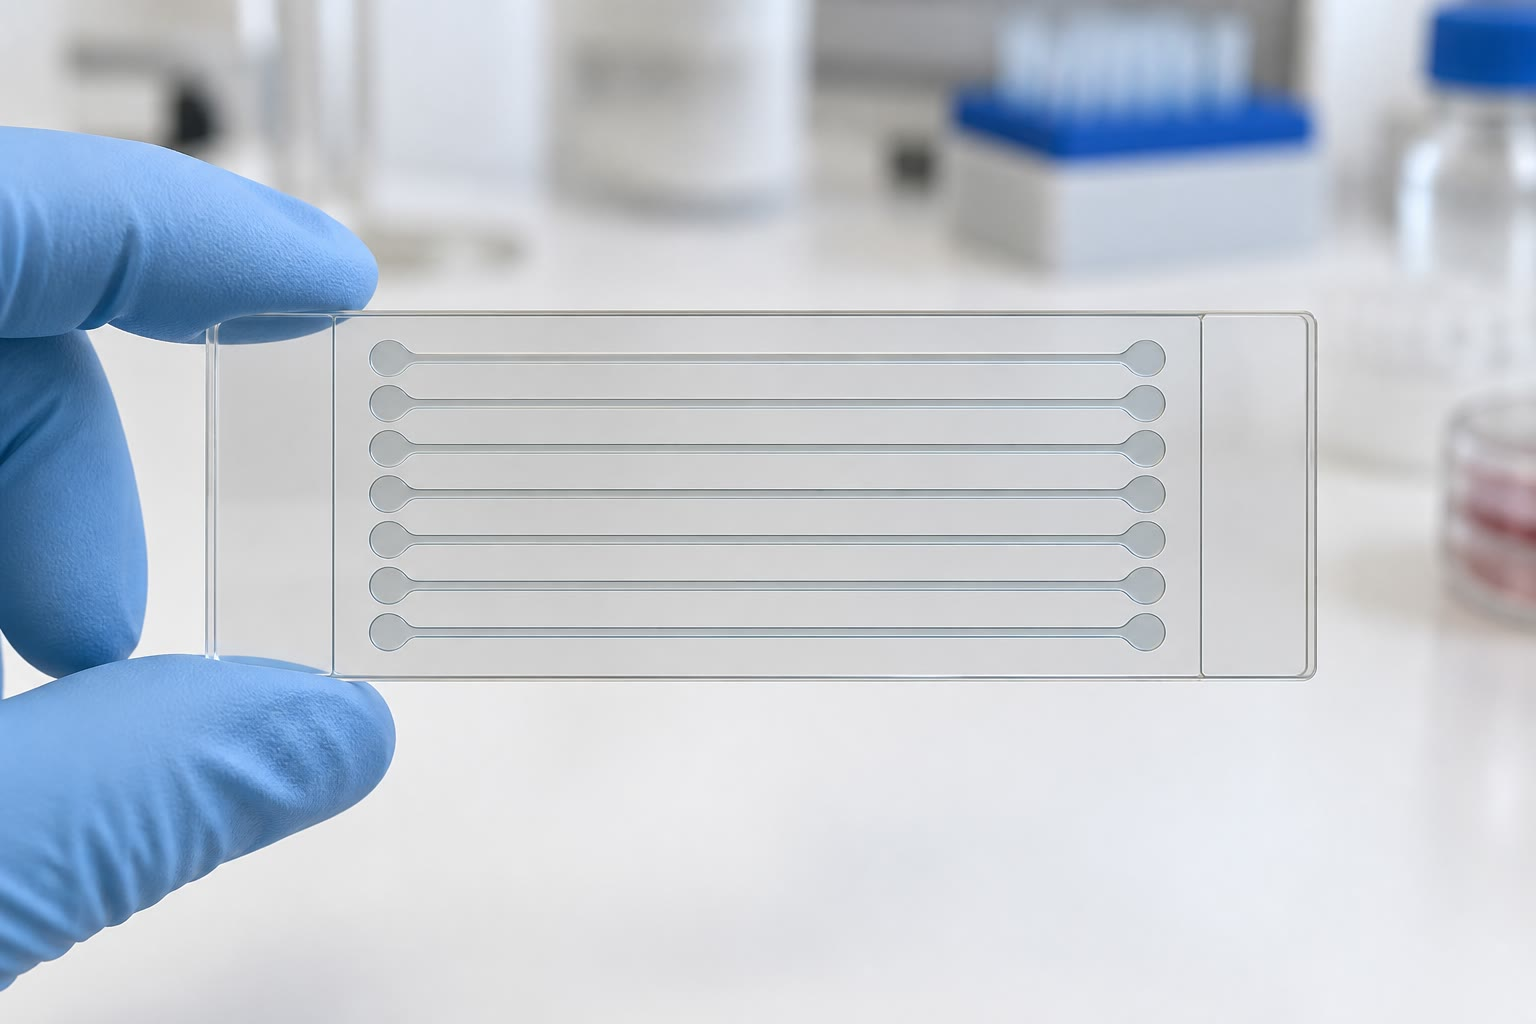
\includegraphics[width=0.46\linewidth]{images/book5/ai/b5-04-flowcell.jpg}\hspace{0.04\linewidth}
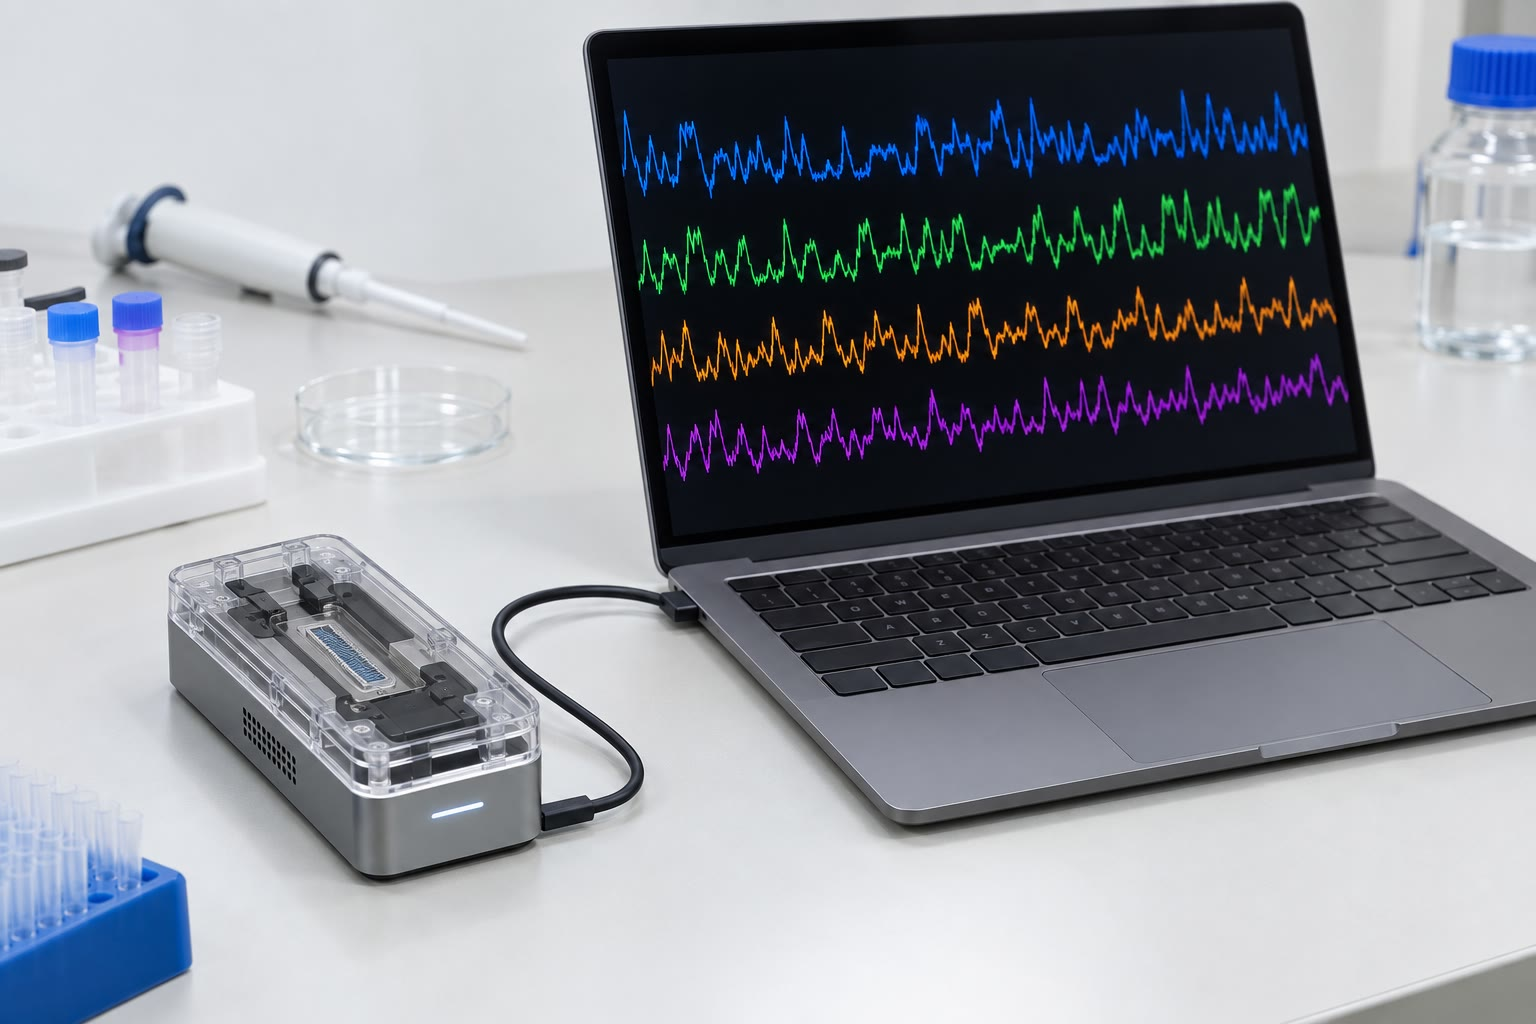
\includegraphics[width=0.46\linewidth]{images/book5/ai/b5-04-nanopore.jpg}

{\small बाएँ: कोई प्रवाह-कोष्ठ, वह काँच की पट्टी जिस पर DNA के अरबों
गुच्छे उगाए जाते हैं और प्रति चक्र एक क्षार पढ़े जाते हैं। दाएँ: जेब
में समाता कोई \omterm{def:b3:genomics:ngs}{नैनोछिद्र} अनुक्रमक, जो अकेले अणुओं को किसी आयनी धारा के
बदलावों के रूप में पढ़ता है।}
\end{omfigure}

\begin{theorem}[किसी शॉटगन परियोजना में आच्छादन और अंतराल]\label{thm:b3:genomics:lander-waterman}
\index{आच्छादन}\index{लैंडर--वॉटरमैन}\index{कॉन्टिग}
मान लीजिए $N$ \omterm{def:b3:genomics:ngs}{वाचन}, जिनमें से हर एक लंबाई $L$ का है, लंबाई $G$ के
किसी जीनोम के साथ-साथ यादृच्छिक स्थितियों पर लिए गए हैं, और $c = NL/G$ को \emph{आच्छादन}
कहिए, यानी किसी क्षार को ढकने वाले \omterm{def:b3:genomics:ngs}{वाचनों} की औसत संख्या। तब कोई दिया
हुआ क्षार \omterm{def:b3:genomics:ngs}{वाचनों} की ऐसी संख्या से ढका होता है जो माध्य $c$ के साथ
पॉइसों है: जीनोम का जो अंश अननुक्रमित रह जाता है वह है
\[
P(\text{अनाच्छादित}) = e^{-c},
\]
और यदि दो \omterm{def:b3:genomics:ngs}{वाचन} तभी अतिव्यापी माने जाएँ जब वे कम-से-कम $T$ क्षार साझा
करें, यानी $\theta = T/L$ हो, तो \emph{कॉन्टिगों} (अतिव्यापी \omterm{def:b3:genomics:ngs}{वाचनों} के
द्वीपों) की प्रत्याशित संख्या है
\[
\text{कॉन्टिग} = N\,e^{-c(1-\theta)},
\]
और उनकी माध्य लंबाई लगभग
$L\,\bigl(e^{c(1-\theta)} - 1\bigr)/c + L\theta$ है।
\end{theorem}
\begin{proof}
\omterm{def:b3:genomics:ngs}{वाचनों} के आरंभ-बिंदु प्रति क्षार $N/G$ घनत्व से यादृच्छिक रूप से पड़ते
हैं। कोई क्षार उन्हीं \omterm{def:b3:genomics:ngs}{वाचनों} से ढका होता है जो उससे पहले के $L$ क्षारों
में आरंभ होते हैं; लंबाई $L$ की किसी खिड़की में आरंभों की संख्या माध्य $LN/G
= c$ के साथ पॉइसों है, और एक भी न होने की प्रायिकता $e^{-c}$ है। कोई
\omterm{def:b3:genomics:ngs}{वाचन} अपने कॉन्टिग का सबसे दायाँ तब होता है जब उसके अपने आरंभ के बाद के
$L - T = L(1-\theta)$ क्षारों में कोई दूसरा \omterm{def:b3:genomics:ngs}{वाचन} आरंभ न हो (बाद में
आरंभ होने वाला \omterm{def:b3:genomics:ngs}{वाचन} उससे $T$ से कम अतिव्यापी होता और जोड़ा नहीं जाता);
वह प्रायिकता $e^{-c(1-\theta)}$ है, और चूँकि हर कॉन्टिग में ठीक एक
सबसे दायाँ \omterm{def:b3:genomics:ngs}{वाचन} होता है, कॉन्टिगों की प्रत्याशित संख्या
$N e^{-c(1-\theta)}$ है। माध्य कॉन्टिग लंबाई $G$ को कॉन्टिगों की
संख्या से भाग देकर, अनाच्छादित अंश का संशोधन करके, निकलती है।
\end{proof}

\begin{example}[कितना पर्याप्त है]\label{ex:b3:genomics:coverage}
$c = 5$ पर अननुक्रमित अंश $e^{-5} = 0.7\,\%$ है --- किसी \qty{3.2}{Gb}
जीनोम के लिए, कुछ दसियों हज़ार अंतरालों में दो करोड़ क्षार। $c = 10$ पर
वह $4.5\times 10^{-5}$ है, कुल मिलाकर \qty{150}{kb}। मानव जीनोमों का
अनुक्रमण नियमित रूप से $c = 30$ पर होता है, आच्छादन-अंतरालों के कारण
नहीं ($e^{-30} \approx 10^{-13}$) बल्कि इसलिए कि हर क्षार को दोनों
गुणसूत्रों में से हर एक पर कई बार पढ़ना पड़ता है ताकि प्रति \omterm{def:b3:genomics:ngs}{वाचन}
$10^{-3}$ त्रुटि-दर के सामने कोई विषमयुग्मजी प्रकारांतर विश्वास से पुकारा
जा सके। जीवाणु जीनोमों का अनुक्रमण इसी कारण और इसलिए भी कि वह सस्ता है,
$c = 50$--$100$ पर होता है। सूत्र यह भी दिखाता है कि आच्छादन क्या ठीक
नहीं कर सकता: किसी \omterm{def:b3:genomics:ngs}{वाचन} से लंबी कोई पुनरावृत्ति वह जगह है जहाँ
अतिव्यापन ग्राफ़ शाखित होता है, और कितने ही छोटे \omterm{def:b3:genomics:ngs}{वाचन} उसे सुलझा नहीं
सकते। दीर्घ \omterm{def:b3:genomics:ngs}{वाचन} इसी के लिए हैं।
\end{example}

\begin{omfigure}
\begin{tikzpicture}
\begin{axis}[
  width=0.7\linewidth, height=5.6cm,
  axis x line=bottom, axis y line=left,
  xmin=0, xmax=12, ymin=0.000001, ymax=1, ymode=log,
  xlabel={आच्छादन $c$}, ylabel={अंश},
  xlabel style={font=\small, at={(axis description cs:0.5,-0.12)}, anchor=north},
  ylabel style={font=\small},
  tick label style={font=\small}, xtick={0,2,4,6,8,10,12},
  clip=false,
]
\addplot[very thick, omDef, domain=0:12, samples=40] {exp(-x)};
\addplot[very thick, omThm, domain=0.3:12, samples=40] {exp(-x*0.8)*x/12};
\node[font=\scriptsize, omDef, anchor=north west] at (axis cs:0.3,0.002) {अनाच्छादित अंश $e^{-c}$};
\node[font=\scriptsize, omThm, anchor=south west] at (axis cs:5.5,0.03) {प्रति वाचन कॉन्टिग $\times\, c/12$, $\theta = 0.2$};
\end{axis}
\end{tikzpicture}

{\small आच्छादन के सामने लैंडर--वॉटरमैन की दो राशियाँ: जीनोम का जो अंश
कभी नहीं पढ़ा जाता वह $e^{-c}$ की तरह गिरता है, और कॉन्टिगों की संख्या
(यहाँ प्रति \omterm{def:b3:genomics:ngs}{वाचन} मापित) कम आच्छादन पर शिखर छूती है और फिर द्वीपों के
मिलते जाने के साथ गिरती है।}
\end{omfigure}

\section{वाचनों से जीनोम तक}

\begin{definition}[संग्रथन और टिप्पणीकरण]\label{def:b3:genomics:assembly}
\index{संग्रथन}\index{स्कैफ़ोल्ड}\index{N50}\index{टिप्पणीकरण}\index{संदर्भ जीनोम}
\emph{संग्रथन} किसी जीनोम को उसके \omterm{def:b3:genomics:ngs}{वाचनों} से अतिव्यापन के सहारे फिर
बनाता है: किसी \emph{अतिव्यापन ग्राफ़} में हर \omterm{def:b3:genomics:ngs}{वाचन} एक शीर्ष है जो उन
\omterm{def:b3:genomics:ngs}{वाचनों} से जुड़ा है जिनसे वह अतिव्यापी है; किसी \emph{दे ब्रॉयन ग्राफ़}
में, जो अरबों छोटे \omterm{def:b3:genomics:ngs}{वाचनों} के लिए काम आता है, हर $k$-मर (लंबाई $k$ का
उपअनुक्रम) एक शीर्ष है और जीनोम उनमें से होकर जाता कोई पथ है। दोनों को
\omterm{def:b3:genomics:ngs}{वाचन} से लंबी पुनरावृत्तियाँ तोड़ देती हैं, जो शाखित पथ देती हैं।
कॉन्टिग युग्मित-सिरे \omterm{def:b3:genomics:ngs}{वाचनों} और दूर-दृष्टि सूचना (दीर्घ \omterm{def:b3:genomics:ngs}{वाचन}, प्रकाशिक
मानचित्र, गुणसूत्र-संपर्क मानचित्र) से क्रम और दिशा में रखकर
\emph{स्कैफ़ोल्ड} बनाए जाते हैं, और स्कैफ़ोल्ड गुणसूत्रों पर रखे जाते
हैं। संग्रथन की गुणवत्ता \emph{N50} से बताई जाती है: वह कॉन्टिग लंबाई
जिसके बराबर या उससे लंबे कॉन्टिगों में संग्रथित क्षारों का आधा भाग हो।
फिर \emph{टिप्पणीकरण} जीन ढूँढ़ता है: जीवाणुओं में, संयोग से लंबे खुले
वाचन-ढाँचे; सुकेंद्रकियों में, अनुक्रम-संकेतों (विच्छेदन स्थल, प्रवर्तक,
कूटक अभिनति), ज्ञात प्रोटीनों से समजातता, और RNA से अनुक्रमित अनुलेखों
को मिलाकर। किसी जाति के लिए परिणाम है कोई \emph{संदर्भ जीनोम}, जिससे उस
जाति का हर बाद का \omterm{def:b3:genomics:ngs}{वाचन} नए सिरे से संग्रथित करने के बजाय संरेखित किया
जाता है।
\end{definition}

\begin{method}[प्रतिदर्श से प्रकारांतरों तक]\label{met:b3:genomics:pipeline}
\index{प्रकारांतर-निर्धारण}
किसी संदर्भ के सामने किसी व्यक्ति के पुनःअनुक्रमण अध्ययन के लिए: (1)
DNA निकालिए, उसे \qtyrange{300}{500}{bp} में खंडित कीजिए, अनुकूलक
जोड़िए (यही \emph{संचय} है); (2) आवश्यक आच्छादन तक अनुक्रमण कीजिए (मानव
जीनोम के लिए 30$\times$, एक्सोम के लिए 100$\times$, जो जीनोम के उस
\qty{1.5}{\%} को पकड़ता है जो प्रोटीन का कूटलेखन करता है); (3) हर \omterm{def:b3:genomics:ngs}{वाचन}
को संदर्भ से संरेखित कीजिए, असंगतियाँ सहते हुए; (4) हर स्थिति पर
\omterm{def:b3:genomics:ngs}{वाचनों} के क्षार गिनिए: जिस स्थिति पर लगभग आधे \omterm{def:b3:genomics:ngs}{वाचन} संदर्भ से असहमत हों
वह कोई विषमयुग्मजी \emph{प्रकारांतर} है, जहाँ लगभग सब असहमत हों वहाँ
समयुग्मजी, जहाँ थोड़े असहमत हों वहाँ कोई त्रुटि; (5) गहराई, क्षार
गुणवत्ता और लड़ी-संतुलन से छानिए; (6) हर प्रकारांतर पर किसी भी जीन पर
उसके प्रभाव (पर्यायी, कुअर्थी, निरर्थक, विच्छेदन, ढाँचा-विस्थापन) और
समष्टि आँकड़ाकोशों में उसकी बारंबारता की टिप्पणी लगाइए; (7) किसी निदान
के लिए, लक्षण-प्ररूप से मेल खाते जीनों में हानिकारक पूर्वानुमानित
दुर्लभ प्रकारांतर रखिए, और \omterm{def:b3:genomics:sanger}{सैंगर अनुक्रमण} से पुष्टि कीजिए।
\end{method}

\section{जीनोम दिखते कैसे हैं}

\begin{proposition}[जीनोम का आकार और जीनों की संख्या]\label{prop:b3:genomics:sizes}
\index{C-मान विरोधाभास}\index{जीनोम आकार}
सुकेंद्रकियों में जीनोम के आकार $10^{5}$ गुने के परास में फैले हैं ---
खमीर के लिए \qty{12}{Mb}, कृमि के लिए \qty{100}{Mb}, मक्खी के लिए
\qty{140}{Mb}, मनुष्य के लिए \qty{3.2}{Gb}, प्याज़ के लिए \qty{16}{Gb},
फेफड़ा-मछली के लिए \qty{130}{Gb}, कुमुदिनी \emph{Paris
japonica} के लिए \qty{150}{Gb} --- जबकि जीनों की संख्याएँ मुश्किल से
$10$ गुने में फैली हैं: खमीर में \num{6000}, कृमि में \num{20000},
मक्खी में \num{14000}, मनुष्य में लगभग \num{20000} प्रोटीन-कूटलेखी
जीन, चावल में \num{40000}। यही \emph{\omterm{prop:b3:genomics:sizes}{C-मान विरोधाभास}} है: जीनोम का आकार
जटिलता नहीं मापता, और न ही जीनों की संख्या। जो बदलता है वह अकूटलेखी
अंतर्वस्तु है --- अंतर्वेशन, स्थानांतरणीय अवयव, उपग्रह पुनरावृत्तियाँ ---
और कोई जीनोम कितने प्रोटीन बना सकता है, यह संख्या उसकी जीन-गणना से कहीं
आगे वैकल्पिक विच्छेदन (\cref{ch:b3:rna-regulation}) और नियमन से बढ़ जाती
है, और जीव की जटिलता अधिकतर वहीं लिखी है। इसके विपरीत जीवाणु जीनोम सघन
हैं और उनका आकार जीन-संख्या के साथ चलता है: लगभग एक जीन प्रति किलोक्षार,
\emph{E.~coli} में \qty{88}{\%} कूटलेखी।
\end{proposition}

\begin{example}[अंतर्वस्तु के हिसाब से मानव जीनोम]\label{ex:b3:genomics:content}
\qty{3.2}{Gb} में से: प्रोटीन-कूटलेखी बहिर्वेशन \qty{1.5}{\%}; जीनों के
अंतर्वेशन और अननुवादित क्षेत्र लगभग \qty{35}{\%}; स्थानांतरणीय अवयव और
उनके जीवाश्म लगभग \qty{45}{\%} --- LINE-1 रेट्रोट्रांसपोज़ॉन
\qty{17}{\%}, Alu अवयव \qty{10}{\%} (किसी \qty{300}{bp} अनुक्रम की दस
लाख से अधिक प्रतियाँ), अंतर्जात रेट्रोवायरस \qty{8}{\%}; खंडीय
द्विगुणन \qty{5}{\%}; सरल पुनरावृत्तियाँ और उपग्रह, गुणसूत्रबिंदुओं
सहित, लगभग \qty{5}{\%}; शेष अनन्य अकूटलेखी अनुक्रम, जहाँ नियामक अवयव
रहते हैं। कोई \numrange{100}{200} जीन अब भी सक्रिय LINE-1 तंत्र का
कूटलेखन करते हैं, और नए प्रवेश लगभग हर बीस जन्मों में एक बार होते हैं।
जीनोम का लगभग \qty{8}{\%} पकड़ में आने योग्य शोधक चयन में है --- बहिर्वेशनों
से कहीं अधिक --- और उसका अधिकांश नियामक है।
\end{example}

\begin{omfigure}
\begin{tikzpicture}[every node/.style={font=\scriptsize}]
  \def\w{12}
  % stacked bar: fractions
  \fill[omThm] (0,0) rectangle (0.18,0.7);
  \fill[omDef!60] (0.18,0) rectangle (4.38,0.7);
  \fill[omProp!70] (4.38,0) rectangle (6.42,0.7);
  \fill[omProp!45] (6.42,0) rectangle (7.62,0.7);
  \fill[omProp!25] (7.62,0) rectangle (9.78,0.7);
  \fill[omMeth!50] (9.78,0) rectangle (10.38,0.7);
  \fill[gray!45] (10.38,0) rectangle (10.98,0.7);
  \fill[gray!15] (10.98,0) rectangle (12,0.7);
  \draw[thick] (0,0) rectangle (12,0.7);
  % labels above/below with leaders
  \draw (0.09,0.7) -- (0.09,1.1); \node[above, align=center] at (0.5,1.1) {बहिर्वेशन\\\qty{1.5}{\%}};
  \node[above] at (2.3,0.75) {जीनों के अंतर्वेशन, UTR: \qty{35}{\%}};
  \node[below, align=center] at (5.4,-0.05) {LINE-1\\\qty{17}{\%}};
  \node[below, align=center] at (7.0,-0.05) {Alu\\\qty{10}{\%}};
  \node[below, align=center] at (8.7,-0.05) {दूसरे ट्रांसपोज़ॉन,\\रेट्रोवायरस \qty{18}{\%}};
  \node[above, align=center] at (10.1,0.75) {खंडीय\\द्विगुणन \qty{5}{\%}};
  \node[below, align=center] at (10.7,-0.05) {उपग्रह\\\qty{5}{\%}};
  \draw[gray] (11.5,0.72) -- (12.0,1.05); \node[above, align=center] at (12.3,1.05) {अन्य अनन्य\\अकूटलेखी};
  \draw[decorate, decoration={brace, amplitude=4pt, mirror}] (4.38,-1.0) -- (9.78,-1.0) node[midway, below=4pt] {स्थानांतरणीय-अवयव से व्युत्पन्न: \qty{45}{\%}};
\end{tikzpicture}

{\small अंतर्वस्तु के हिसाब से मानव जीनोम, मापानुसार। प्रोटीन-कूटलेखी
बहिर्वेशन (लाल) एक पतली फाँक हैं; जीनोम का लगभग आधा भाग स्थानांतरणीय
अवयवों से उतरा है।}
\end{omfigure}

\begin{definition}[तुलनात्मक जीनोमिकी]\label{def:b3:genomics:comparative}
\index{ऑर्थोलॉग}\index{पैरालॉग}\index{सहविन्यास}\index{संरक्षित अकूटलेखी अवयव}\index{पूर्ण-जीनोम द्विगुणन}
दो जातियों के वे जीन जो उनके साझा पूर्वज के एक ही जीन से उतरे हैं
\emph{ऑर्थोलॉग} हैं; किसी एक जाति के भीतर किसी द्विगुणन से उतरे जीन
\emph{पैरालॉग} हैं। गुणसूत्र के वे खंड जिनमें जातियों के बीच जीन-क्रम
संरक्षित है \emph{सहविन्यासी} हैं; सहविन्यास से किसी जीन को एक जीनोम
में दूसरे जीनोम में उसकी स्थिति से ढूँढ़ा जा सकता है और वे
पुनर्विन्यास उजागर होते हैं जो दो गुणसूत्र-प्ररूपों को अलग करते हैं
(मनुष्य और चूहे के बीच लगभग \num{1000})। दूर की जातियों के पार संरक्षित
वे अनुक्रम जो किसी प्रोटीन का कूटलेखन नहीं करते ---
\emph{संरक्षित अकूटलेखी अवयव}, जिनमें से कुछ मनुष्य और मछली के बीच
\qty{200}{bp} तक क्षार-दर-क्षार अतिसंरक्षित हैं --- अधिकतर परिवर्धन-जीनों
के संवर्धक हैं। \emph{पूर्ण-जीनोम द्विगुणनों} ने वंशक्रमों के इतिहास
पर छाप छोड़ी है: कशेरुकियों के उद्गम पर दो बारियाँ (अकशेरुकियों के एक
गुच्छे के सामने स्तनधारियों के चार Hox गुच्छे), सैल्मन-कुल के पूर्वज
में एक, खमीर के वंशक्रम में एक, सपुष्प पौधों में कई; द्विगुणित जीन
अधिकतर करोड़ों वर्षों में खो जाते हैं, और जो बचते हैं उनका प्रकार्य
अलग हो जाता है।
\end{definition}

\begin{example}[मनुष्य और चिंपैंज़ी]\label{ex:b3:genomics:chimp}
संरेखित एकल-प्रति अनुक्रम मनुष्य और चिंपैंज़ी के बीच क्षारों के
\qty{1.2}{\%} पर भिन्न है --- कोई \num{35} लाख प्रतिस्थापन --- और ऐसे
अंतर्वेशनों तथा विलोपनों से भी जो मिलकर हर जीनोम के और \qty{3}{\%}
बनते हैं। दो मनुष्य हज़ार में लगभग एक क्षार पर भिन्न होते हैं, यानी कोई
\numrange{4}{5} लाख स्थलों पर, और साथ में कुछ हज़ार संरचनात्मक
प्रकारांतर; दो चिंपैंज़ी, जिनकी समष्टि अधिक समय तक बड़ी रही है, इससे
कुछ अधिक पर। कोई बच्चा लगभग \num{70} ऐसे नए उत्परिवर्तन ढोता है जो
दोनों जनकों में नहीं हैं, उनमें से चार-पंचमांश पिता से, और यह संख्या
पिता की आयु के प्रति वर्ष लगभग दो से बढ़ती है --- शुक्राणुजनन के अनेक
विभाजनों पर लगाया गया \cref{ch:b3:dna-repair} का अंकगणित।
\end{example}

\section{जीनोम और लक्षण}

\begin{definition}[जीनोम-व्यापी सहचर्य]\label{def:b3:genomics:gwas}
\index{जीनोम-व्यापी सहचर्य अध्ययन}\index{एकल-न्यूक्लियोटाइड बहुरूपता}\index{बहुजीनी अंक}
\emph{एकल-न्यूक्लियोटाइड बहुरूपता} (SNP) ऐसी स्थिति है जिस पर दो क्षार
किसी समष्टि के कम-से-कम \qty{1}{\%} में आते हैं; मनुष्यों में लगभग एक
करोड़ सामान्य हैं। कोई \emph{जीनोम-व्यापी सहचर्य अध्ययन} (GWAS) किसी
रोग वाले हज़ारों और बिना रोग वाले हज़ारों लोगों में लाखों SNP का
जीन-प्ररूपण करता है और हर SNP पर पूछता है कि कोई एक युग्मविकल्पी
रोगियों में अधिक बारंबार है या नहीं। चूँकि दस लाख परीक्षण किए जाते हैं,
कोई परिणाम तभी गिना जाता है जब वह लगभग $5\times 10^{-8}$ की
सार्थकता-देहली से नीचे हो ($0.05$ को प्रभावी रूप से स्वतंत्र दस लाख
परीक्षणों से भाग देकर)। सहचारी SNP किसी क्षेत्र को चिह्नित करते हैं,
किसी कारक प्रकारांतर को नहीं, क्योंकि पड़ोसी युग्मविकल्पी दसियों
किलोक्षार तक साथ-साथ चलते हैं (सहलग्नता असंतुलन)। अधिकांश सामान्य रोगों
के लिए सहचारी युग्मविकल्पी जोखिम को कुछ प्रतिशत ही खिसकाते हैं और
अधिकतर नियामक अनुक्रम में पड़ते हैं; उनका संयुक्त प्रभाव, हज़ारों SNP पर
जोड़कर किसी \emph{बहुजीनी अंक} के रूप में, वंशागतता का एक अंश समझाता है
और जोखिम का पूर्वानुमान लगभग उतना ही अच्छा करता है जितना कुल-इतिहास।
\end{definition}

\begin{remark}[जीनोमिकी ने क्या दिया और क्या नहीं]\label{rem:b3:genomics:delivered}
अनुक्रमण वहाँ निर्णायक रहा है जहाँ किसी एक जीन का बड़ा प्रभाव है: कई
हज़ार मेंडेली रोगों के जीन मिल चुके हैं, और किसी अनिदानित विकार वाले
बच्चे के एक्सोम का अनुक्रमण लगभग एक-तिहाई स्थितियों में निदान देता है।
कर्कट जीनोम बताते हैं कि कोई अर्बुद कौन-से चालक ढोता है और कौन-सी औषधें
काम कर सकती हैं (\cref{ch:b3:cancer-biology}); रोगजनक जीनोम प्रकोपों को
प्रजाति-दर-प्रजाति खोज निकालते हैं (\cref{ch:b3:bacteriology}); प्राचीन
जीनोमों ने मानव प्रागितिहास फिर से लिखा है और दिखाया है कि अफ़्रीका के
बाहर के लोग लगभग \qty{2}{\%} नियंडरथाल DNA ढोते हैं। सामान्य रोगों के
लिए --- मधुमेह, हृद्रोग, मनोविदलता --- जीनोमिकी ने हज़ारों छोटे प्रभाव
दिए हैं और थोड़ी ही क्रियाविधियाँ, और किसी स्वस्थ व्यक्ति के जीनोम से
पूर्वानुमान का वादा अब भी विनम्र है। जीनोम पुर्ज़ों की सूची है; पुर्ज़े
आपस में कैसे काम करते हैं, वह जीवविज्ञान उससे पढ़ा नहीं जाता।
\end{remark}

\section{अभ्यास}

\begin{exercise}[$\star$]\label{exo:b3:genomics:1}
समझाइए कि कोई \omterm{def:b3:genomics:sanger}{डाइडिऑक्सीन्यूक्लियोटाइड} बढ़ती DNA शृंखला को क्यों समाप्त
कर देता है, और किसी सैंगर अभिक्रिया में हर न्यूक्लियोटाइड के सामान्य
और डाइडिऑक्सी दोनों रूप क्यों होने चाहिए।
\end{exercise}

\begin{exercise}[$\star$]\label{exo:b3:genomics:2}
कोई बारी $4\times 10^{8}$ युग्मित \omterm{def:b3:genomics:ngs}{वाचन} देती है, हर एक $2\times \qty{150}{bp}$ का।
इससे किसी \qty{3.2}{Gb} मानव जीनोम का कितना आच्छादन मिलता है? किसी
\qty{5}{Mb} जीवाणु जीनोम का?
\end{exercise}

\begin{exercise}[$\star$]\label{exo:b3:genomics:3}
कॉन्टिग, \omterm{def:b3:genomics:assembly}{स्कैफ़ोल्ड} और \omterm{def:b3:genomics:assembly}{N50} को परिभाषित कीजिए। \qty{100}{Mb} के किसी
\omterm{def:b3:genomics:assembly}{संग्रथन} में \qty{8}{Mb} के दस कॉन्टिग और \qty{10}{kb} के \num{2000} हैं।
उसका \omterm{def:b3:genomics:assembly}{N50} क्या है?
\end{exercise}

\begin{exercise}[$\star$]\label{exo:b3:genomics:4}
\omterm{prop:b3:genomics:sizes}{C-मान विरोधाभास} को दो उदाहरणों के साथ बताइए, और कहिए कि बड़े जीनोमों के
अतिरिक्त DNA का अधिकांश किससे बनता है।
\end{exercise}

\begin{exercise}[$\star\star$]\label{exo:b3:genomics:5}
\cref{thm:b3:genomics:lander-waterman} का उपयोग करते हुए वह आच्छादन
निकालिए जो दस लाख में अधिक-से-अधिक एक क्षार अननुक्रमित छोड़े, और
\qty{150}{bp} \omterm{def:b3:genomics:ngs}{वाचनों} तथा \qty{30}{bp} न्यूनतम अतिव्यापन के साथ $c = 8$
पर पढ़े गए किसी \qty{5}{Mb} जीनोम के लिए कॉन्टिगों की प्रत्याशित संख्या।
\end{exercise}

\begin{exercise}[$\star\star$]\label{exo:b3:genomics:6}
कोई विषमयुग्मजी प्रकारांतर $30$ \omterm{def:b3:genomics:ngs}{वाचनों} से ढका है। यह मानते हुए कि हर
\omterm{def:b3:genomics:ngs}{वाचन} प्रायिकता $1/2$ से किसी भी युग्मविकल्पी को दिखाता है, इसकी
प्रायिकता क्या है कि $8$ से कम \omterm{def:b3:genomics:ngs}{वाचन} प्रकारांतर युग्मविकल्पी दिखाएँ
(जिससे उसे त्रुटियाँ समझ लिया जाए)? माध्य $15$ और मानक विचलन
$\sqrt{7.5}$ के साथ प्रसामान्य सन्निकटन का उपयोग कीजिए। $30\times$ मानक
क्यों है?
\end{exercise}

\begin{exercise}[$\star\star$]\label{exo:b3:genomics:7}
किसी जीनोम में \qty{6}{kb} की कोई पुनरावृत्ति \num{500} प्रतियों में
है। समझाइए कि \qty{150}{bp} \omterm{def:b3:genomics:ngs}{वाचनों} से बना कोई \omterm{def:b3:genomics:assembly}{संग्रथन} उसे क्यों ढहा
देता है, परिणामी ग्राफ़ कैसा दिखता है, और कितनी वाचन-लंबाई उसे सुलझा देगी।
\end{exercise}

\begin{exercise}[$\star\star$]\label{exo:b3:genomics:8}
दो मनुष्य हज़ार में एक क्षार पर भिन्न हैं। उनके एक्सोमों
(\qty{48}{Mb} कूटलेखी अनुक्रम) में कितने अंतर होंगे? यदि कूटलेखी अंतरों
में से दो-तिहाई पर्यायी या सौम्य हों और शेष किसी प्रोटीन को बदलते हों,
तो एक व्यक्ति दूसरे के सापेक्ष कितने प्रोटीन-बदलने वाले प्रकारांतर ढोता है?
\end{exercise}

\begin{exercise}[$\star\star$]\label{exo:b3:genomics:9}
कोई GWAS $10^{6}$ SNP का परीक्षण देहली $p < 5\times 10^{-8}$ पर करता
है। यदि कोई भी SNP वस्तुतः सहचारी न हो तो कितने मिथ्या धनात्मक
प्रत्याशित हैं? कोई SNP युग्मविकल्पी \qty{2}{\%} बारंबारता वाले किसी
रोग का जोखिम बढ़ाकर \qty{2.3}{\%} कर देता है। समझाइए कि ऐसा प्रभाव
हज़ार लोगों के अध्ययन में क्यों पकड़ में नहीं आता और किसी व्यक्ति के लिए
क्यों बेकार है, फिर भी वह किसी क्रियाविधि की ओर क्यों इशारा कर सकता है।
\end{exercise}

\begin{exercise}[$\star\star\star$]\label{exo:b3:genomics:10}
जीवाणु जीनोम लगभग \qty{88}{\%} कूटलेखी हैं; मानव जीनोम \qty{1.5}{\%}।
इस अंतर के लिए तीन परिकल्पनाएँ दीजिए --- समष्टि-आनुवंशिक, संरचनात्मक
और नियामक --- और हर एक के लिए कोई ऐसा जीनोमी प्रेक्षण जो उसका समर्थन
करता हो या उसे कमज़ोर करता हो।
\end{exercise}

\begin{exercise}[$\star\star\star$]\label{exo:b3:genomics:11}
दो भिन्न लंबाइयों के मिश्रित \omterm{def:b3:genomics:ngs}{वाचनों} के लिए लैंडर--वॉटरमैन कॉन्टिग-गणना
व्युत्पन्न कीजिए: $N_{1}$ छोटे \omterm{def:b3:genomics:ngs}{वाचन}, लंबाई $L_{1}$ के, और $N_{2}$
दीर्घ \omterm{def:b3:genomics:ngs}{वाचन}, लंबाई $L_{2}$ के, अतिव्यापन उसी न्यूनतम $T$ से गिने गए।
(हर \omterm{def:b3:genomics:ngs}{वाचन} को अपने कॉन्टिग का सबसे दायाँ मानिए यदि उसकी अपनी लंबाई घटा
$T$ के भीतर किसी भी प्रकार का कोई \omterm{def:b3:genomics:ngs}{वाचन} आरंभ न हो।) दिखाइए कि थोड़े
दीर्घ \omterm{def:b3:genomics:ngs}{वाचन} कॉन्टिग-गणना उतने ही क्षारों वाले छोटे \omterm{def:b3:genomics:ngs}{वाचनों} से अधिक घटाते हैं।
\end{exercise}

\begin{exercise}[$\star\star\star$]\label{exo:b3:genomics:12}
यह तर्क दिया जाता है कि स्तनधारियों के चार Hox गुच्छे कशेरुकियों के आधार
पर हुए \omterm{def:b3:genomics:comparative}{पूर्ण-जीनोम द्विगुणन} की दो बारियों से एक ही गुच्छे से उतरे हैं।
बताइए कि यह परिकल्पना जीनोम भर \omterm{def:b3:genomics:comparative}{पैरालॉगों} का कौन-सा प्रतिरूप, और
लैम्प्रे तथा अकशेरुकी कॉर्डेटों के जीनोमों में कौन-सा प्रतिरूप,
पूर्वानुमानित करती है, और उसे अकेले गुच्छे के दो स्वतंत्र द्विगुणनों से
कैसे अलग किया जाएगा।
\end{exercise}

\section{समस्या: एक ही मशीन पर दो जीनोम}

\begin{problem}[{सप्तांत समस्या --- एक ही बारी में अनुक्रमित एक जीवाणु और
एक मनुष्य: वाचनों का बँटवारा, आच्छादन तथा अंतरालों की गणना, कॉन्टिगों
की गिनती, त्रुटि-दर के सामने विषमयुग्मजी प्रकारांतरों का निर्धारण, मानव
जीनोम की अंतर्वस्तु का तौल, और किसी सहचर्य अध्ययन का आकार, जिसका अंत
कम आच्छादन पर कॉन्टिग-गणना, प्रकारांतर-निर्धारण को सुरक्षित बनाने वाले
आच्छादन और किसी बच्चे में नए उत्परिवर्तनों की संख्या पर होता है}]
\label{pb:b3:genomics:1}
आँकड़े: एक बारी \qty{150}{bp} के $6\times 10^{8}$ \omterm{def:b3:genomics:ngs}{वाचन} देती है। कोई
जीवाणु जीनोम \qty{4.6}{Mb} का है; मानव जीनोम \qty{3.2}{Gb}
(अगुणित)। न्यूनतम अतिव्यापन $T = \qty{30}{bp}$। प्रति \omterm{def:b3:genomics:ngs}{वाचन} प्रति क्षार
त्रुटि-दर $10^{-3}$। मानव कूटलेखी अनुक्रम \qty{48}{Mb}; जीनोम
\qty{45}{\%} ट्रांसपोज़ॉन-व्युत्पन्न है, जिसमें \qty{300}{bp} की $1.1$
करोड़ Alu प्रतियाँ हैं। दो मनुष्य \num{1000} में एक स्थल पर भिन्न हैं।
प्रति क्षार प्रति पीढ़ी उत्परिवर्तन-दर $1.2\times 10^{-8}$।

\medskip
\noindent\textbf{भाग I --- जीवाणु।}
\begin{enumerate}
  \item जीवाणु को बारी का \qty{0.2}{\%} दिया जाता है। कितने \omterm{def:b3:genomics:ngs}{वाचन}, और
        कितना आच्छादन?
  \item उसके जीनोम का कितना अंश अननुक्रमित है? वह कितने क्षार हुए?
  \item $\theta$ और कॉन्टिगों की प्रत्याशित संख्या निकालिए।
  \item किसी पहले के प्रायोगिक चरण में केवल \num{30000} \omterm{def:b3:genomics:ngs}{वाचन} काम में
        आए थे। आच्छादन, अनाच्छादित अंश और कॉन्टिग-संख्या?
  \item जीनोम में किसी \qty{5}{kb} rRNA प्रकार्यगुच्छ की \num{7}
        प्रतियाँ हैं। बताइए कि \omterm{def:b3:genomics:assembly}{संग्रथन} में उनके साथ क्या होता है और
        अकेले इसी से कितने कॉन्टिग-सिरे बनते हैं।
  \item जीवाणु में लगभग एक जीन प्रति किलोक्षार है। कितने जीन, और यदि
        जीनोम का \qty{88}{\%} कूटलेखी हो तो माध्य जीन-लंबाई क्या है?
\end{enumerate}

\medskip
\noindent\textbf{भाग II --- मनुष्य।}
\begin{enumerate}[resume]
  \item बारी का शेष भाग एक मानव जीनोम को जाता है। द्विगुणित जीनोम का
        प्रति अगुणित प्रति के हिसाब से आच्छादन (यानी कुल क्षारों को
        \qty{3.2}{Gb} से भाग देकर)?
  \item किसी विषमयुग्मजी स्थल पर दोनों युग्मविकल्पियों में से हर एक
        लगभग आधे \omterm{def:b3:genomics:ngs}{वाचनों} से ढका होता है। प्रश्न 7 के आच्छादन के साथ हर
        युग्मविकल्पी को दिखाने वाले \omterm{def:b3:genomics:ngs}{वाचनों} की प्रत्याशित संख्या क्या है?
  \item कोई त्रुटि किसी \omterm{def:b3:genomics:ngs}{वाचन} में प्रायिकता $10^{-3}$ से कोई गलत क्षार
        दिखाती है। $c$ \omterm{def:b3:genomics:ngs}{वाचनों} से ढके किसी समयुग्मजी स्थल पर किसी विशेष
        गलत क्षार को दिखाने वाले \omterm{def:b3:genomics:ngs}{वाचनों} की प्रत्याशित संख्या क्या है
        (हर एक $10^{-3}/3$)? इस आच्छादन पर ``प्रकारांतर तभी पुकारिए जब
        कम-से-कम $3$ \omterm{def:b3:genomics:ngs}{वाचन} और कम-से-कम \qty{20}{\%} \omterm{def:b3:genomics:ngs}{वाचन} उसे दिखाएँ''
        वाला नियम त्रुटियों को क्यों अस्वीकार कर देता है?
  \item कोई मनुष्य कितने विषमयुग्मजी स्थल ढोता है (दो यादृच्छिक
        जीनोमों के अंतरों का मोटे तौर पर आधा हर एक में पड़ता है:
        \num{1500} में एक स्थल लीजिए)? कूटलेखी अनुक्रम में कितने?
  \item \omterm{def:b3:genomics:ngs}{वाचन} किसी संदर्भ से संरेखित किए जाते हैं। समझाइए कि Alu अवयवों
        से आए \omterm{def:b3:genomics:ngs}{वाचन} प्रायः गलत प्रति पर क्यों संरेखित होते हैं और उनके
        भीतर प्रकारांतर-निर्धारण पर इसका क्या परिणाम होता है।
  \item किसी बच्चे का अनुक्रमण दोनों जनकों के साथ होता है। आप कितने नए
        उत्परिवर्तन की अपेक्षा करते हैं? इस आच्छादन पर बच्चे में कितने
        \omterm{def:b3:genomics:ngs}{वाचनों} को ऐसा प्रकारांतर दिखाना चाहिए जो \emph{दोनों} जनकों में
        अनुपस्थित हो, ताकि उस पर विश्वास किया जाए, और जनकों का आच्छादन
        बच्चे के आच्छादन जितना ही महत्वपूर्ण क्यों है?
  \item कोई चिकित्सकीय प्रयोगशाला एक्सोम (\qty{48}{Mb}) पकड़ती है और
        उसका $100\times$ पर अनुक्रमण करती है। इसमें कितने \omterm{def:b3:genomics:ngs}{वाचन} लगते
        हैं, और यह प्रति रोगी $28\times$ पर किसी जीनोम से सस्ता क्यों
        है, जबकि उसका आच्छादन अधिक है?
\end{enumerate}

\medskip
\noindent\textbf{भाग III --- किसी जीनोम की अंतर्वस्तु।}
\begin{enumerate}[resume]
  \item मानव जीनोम का कितना अंश Alu है, और प्रश्न 7 के \omterm{def:b3:genomics:ngs}{वाचनों} में से
        कितने Alu अवयवों से आते हैं?
  \item संदर्भ \qty{3.2}{Gb} का है पर किसी द्विगुणित कोशिका में
        \qty{6.4}{Gb} है; और \qty{16}{Gb} वाले किसी प्याज़ में लगभग
        \num{60000} जीन हैं। यदि उसके जीनों में औसतन \qty{1.5}{kb}
        कूटलेखी अनुक्रम हो तो प्याज़ के जीनोम का कूटलेखी अंश क्या है?
  \item मनुष्य और चिंपैंज़ी संरेखित क्षारों के \qty{1.2}{\%} पर भिन्न
        हैं। \qty{2.9}{Gb} संरेखणीय अनुक्रम में यह कितने प्रतिस्थापन
        हुए? $6.5$ करोड़ वर्षों में दोनों वंशक्रमों के बीच बराबर बाँटा
        जाए तो इससे प्रति क्षार प्रति वर्ष और $25$ वर्ष की प्रति पीढ़ी
        कौन-सी उत्परिवर्तन-दर निकलती है? आँकड़ों में दिए गए सीधे मापन
        से तुलना कीजिए।
  \item कशेरुकियों के दो जीनोम-द्विगुणनों से हर पूर्वज जीन की चार तक
        प्रतियाँ मिलनी चाहिए। मनुष्यों में लगभग \num{20000} जीन हैं और
        अकशेरुकी कॉर्डेट \emph{Ciona} में लगभग \num{16000}। इस
        परिकल्पना पर कि पूर्वज के पास \num{16000} थे, द्विगुणों का
        कितना अंश खो चुका है?
  \item समझाइए कि जीन-संख्या जीव की जटिलता का खराब माप क्यों है, और
        तर्क के रूप में \cref{ch:b3:rna-regulation} की वैकल्पिक
        विच्छेदन-गणना लीजिए।
  \item जीनोम का \qty{8}{\%} शोधक चयन में है पर केवल \qty{1.5}{\%}
        प्रोटीन का कूटलेखन करता है। शेष क्या होने की संभावना है, और आप
        किसी एक संभावित अवयव का परीक्षण कैसे करेंगे?
\end{enumerate}

\medskip
\noindent\textbf{भाग IV --- एक सहचर्य अध्ययन।}
\begin{enumerate}[resume]
  \item $10^{6}$ SNP का परीक्षण होता है। $0.05$ की कुल-परिवार त्रुटि के
        लिए बोन्फ़ेरोनी देहली बताइए, और $p < 10^{-5}$ पर मिथ्या
        धनात्मकों की प्रत्याशित संख्या।
  \item किसी रोग की व्यापकता \qty{1}{\%} है। बारंबारता $0.3$ का कोई
        जोखिम युग्मविकल्पी संभावना-अनुपात \qty{5}{\%} बढ़ा देता है। दो
        प्रतियाँ, एक प्रति और कोई प्रति न ढोने वाले का रोग-जोखिम
        निकालिए, अवाहक का जोखिम \qty{0.9}{\%} लेकर। (संभावना-अनुपात
        गुणा कीजिए।)
  \item ऐसे दो सौ युग्मविकल्पी मिलते हैं। समझाइए कि \omterm{def:b3:genomics:gwas}{बहुजीनी अंक} क्या
        है, और ऊपरी \qty{1}{\%} में पड़े किसी व्यक्ति का अंक कई गुना
        जोखिम के तुल्य क्यों हो सकता है जबकि हर युग्मविकल्पी लगभग कुछ
        नहीं करता।
  \item समझाइए कि सार्थकता तक पहुँचा कोई SNP प्रायः कारक प्रकारांतर
        क्यों नहीं होता, और उस क्षेत्र में कारक प्रकारांतर की पहचान
        कौन-सा प्रयोग करेगा।
  \item \num{40000} वर्ष पुरानी किसी हड्डी के किसी प्राचीन जीनोम का
        $c = 0.5$ पर अनुक्रमण होता है। उसका कितना अंश पढ़ा जाता है?
        यह फिर भी समष्टि-इतिहास के वे प्रश्न क्यों हल कर सकता है जो
        अकेला कोई आधुनिक जीनोम नहीं कर सकता?
  \item सारांश दीजिए: प्रायोगिक \omterm{def:b3:genomics:assembly}{संग्रथन} में कॉन्टिगों की संख्या
        (प्रश्न~4), वह प्रति अगुणित जीनोम आच्छादन जो प्रति
        युग्मविकल्पी लगभग $15$ \omterm{def:b3:genomics:ngs}{वाचन} देता है (प्रश्न~7--8), और किसी
        बच्चे में नए उत्परिवर्तनों की संख्या (प्रश्न~12)।
\end{enumerate}
\end{problem}
